\documentclass[10pt,a4paper]{article}
% Shared formal submission style for CoExist Alert PDFs.
\usepackage[a4paper,margin=0.72in,headheight=30pt,footskip=32pt]{geometry}
\usepackage[utf8]{inputenc}
\usepackage[T1]{fontenc}
\usepackage{lmodern}
\usepackage{microtype}
\usepackage[dvipsnames,table]{xcolor}
\usepackage{graphicx}
\usepackage{booktabs}
\usepackage{tabularx}
\usepackage{array}
\usepackage{enumitem}
\usepackage{titlesec}
\usepackage{tcolorbox}
\tcbuselibrary{skins,breakable}
\usepackage{fancyhdr}
\usepackage{pdflscape}
\usepackage[hidelinks]{hyperref}
\usepackage{tikz}
\usetikzlibrary{arrows.meta,positioning,calc,fit,shapes.geometric,backgrounds}

\definecolor{BrandColor}{HTML}{3FADA8}
\definecolor{AccentColor}{HTML}{277A75}
\definecolor{InkColor}{HTML}{333333}
\definecolor{SoftGray}{HTML}{F5F6F6}
\definecolor{LineGray}{HTML}{D9E1E1}
\definecolor{DangerColor}{HTML}{8D2A2A}
\definecolor{WarningColor}{HTML}{8A4F14}
\definecolor{SuccessColor}{HTML}{18794D}

\hypersetup{
  colorlinks=true,
  linkcolor=AccentColor,
  urlcolor=AccentColor
}

\pagestyle{fancy}
\fancyhf{}
\renewcommand{\headrulewidth}{0.45pt}
\renewcommand{\footrulewidth}{0.45pt}
\fancyhead[L]{\scriptsize\sffamily\bfseries CoExist Alert \textbar\ Silver Flag CSR Challenge}
\fancyhead[R]{\scriptsize\sffamily Team GitBoosters}
\fancyfoot[L]{\scriptsize\sffamily Yash Kumar Vaibhav \textbar\ IIIT Delhi}
\fancyfoot[C]{\scriptsize\sffamily Varnika Pulipati \textbar\ IIITDM Jabalpur}
\fancyfoot[R]{\scriptsize\sffamily Adeesh Jain \textbar\ BITS Pilani Goa \quad \thepage}

\titleformat{\section}
  {\normalfont\Large\sffamily\bfseries\color{BrandColor}}
  {\thesection}{0.6em}{}[{\vspace{0.1cm}\color{BrandColor}\titlerule[0.3pt]}]

\titleformat{\subsection}
  {\normalfont\large\sffamily\bfseries\color{AccentColor}}
  {\thesubsection}{0.6em}{}

\titleformat{\subsubsection}
  {\normalfont\normalsize\sffamily\bfseries\color{AccentColor}}
  {}{0em}{}

\titlespacing*{\section}{0pt}{0.8em}{0.45em}
\titlespacing*{\subsection}{0pt}{0.65em}{0.25em}
\titlespacing*{\subsubsection}{0pt}{0.5em}{0.2em}
\setlist[itemize]{leftmargin=1.2em, topsep=2pt, itemsep=1pt}
\setlist[enumerate]{leftmargin=1.4em, topsep=2pt, itemsep=1pt}
\setlength{\parindent}{0pt}
\setlength{\parskip}{4pt}

\newtcolorbox{summarybox}[1][Summary]{
  enhanced, breakable, colback=BrandColor!8, colframe=BrandColor,
  arc=3pt, boxrule=0.65pt, left=8pt, right=8pt, top=6pt, bottom=6pt,
  borderline west={3pt}{0pt}{BrandColor},
  title={#1}, coltitle=InkColor, fonttitle=\bfseries\sffamily
}

\newtcolorbox{decisionbox}[1]{
  enhanced, breakable, colback=gray!4, colframe=BrandColor!70!black,
  arc=2pt, boxrule=0.45pt, left=7pt, right=7pt, top=5pt, bottom=5pt,
  title={#1}, coltitle=white, fonttitle=\bfseries\sffamily,
  colbacktitle=BrandColor!70!black
}

\newcommand{\docheader}[2]{
  \begin{center}
    
\includegraphics[height=1.35cm]{../public/coexist-logo.png}\\[0.25cm]
    {\huge\sffamily\bfseries\color{BrandColor} #1}\\[0.15cm]
    {\large\sffamily #2}\\[0.15cm]
    {\small\sffamily\color{gray} Code with Cisco \textbar\ Silver Flag CSR Challenge \textbar\ Mission 3: Human-Animal Coexistence}\\[0.2cm]
  \end{center}
  \vspace{-0.2cm}
  {\color{BrandColor}\hrule height 0.6pt}
  \vspace{0.25cm}
}

\tikzset{
  box/.style={draw=LineGray, rounded corners=3pt, fill=white, align=center, inner sep=6pt, font=\scriptsize\sffamily},
  brandbox/.style={box, draw=BrandColor, fill=BrandColor!8},
  stagebox/.style={box, draw=AccentColor, fill=BrandColor!10},
  dangerbox/.style={box, draw=DangerColor, fill=DangerColor!7},
  arrow/.style={-Latex, thick, draw=AccentColor},
  mutedarrow/.style={-Latex, draw=gray!65}
}

\newcolumntype{Y}{>{\raggedright\arraybackslash}X}


\begin{document}

\docheader{Architecture Diagrams}{CoExist Alert}

\begin{summarybox}[Architecture Read]
These diagrams show the four views reviewers need most: system components, detection-to-warning sequence, escalation and ownership workflow, and runtime deployment. The PDF embeds Mermaid-rendered vector diagrams generated from the companion sources under \texttt{docs/diagrams/}.
\end{summarybox}

\begin{decisionbox}{Reading note}
Field sensors are simulated in this proof of concept and are labeled that way in the UI and diagrams. Demo controls are a user-facing surface: they can trigger the ingest API for rehearsal, but they are not a field sensor node.
\end{decisionbox}

\clearpage
\section{System Components}

\begin{center}
\makebox[\textwidth][c]{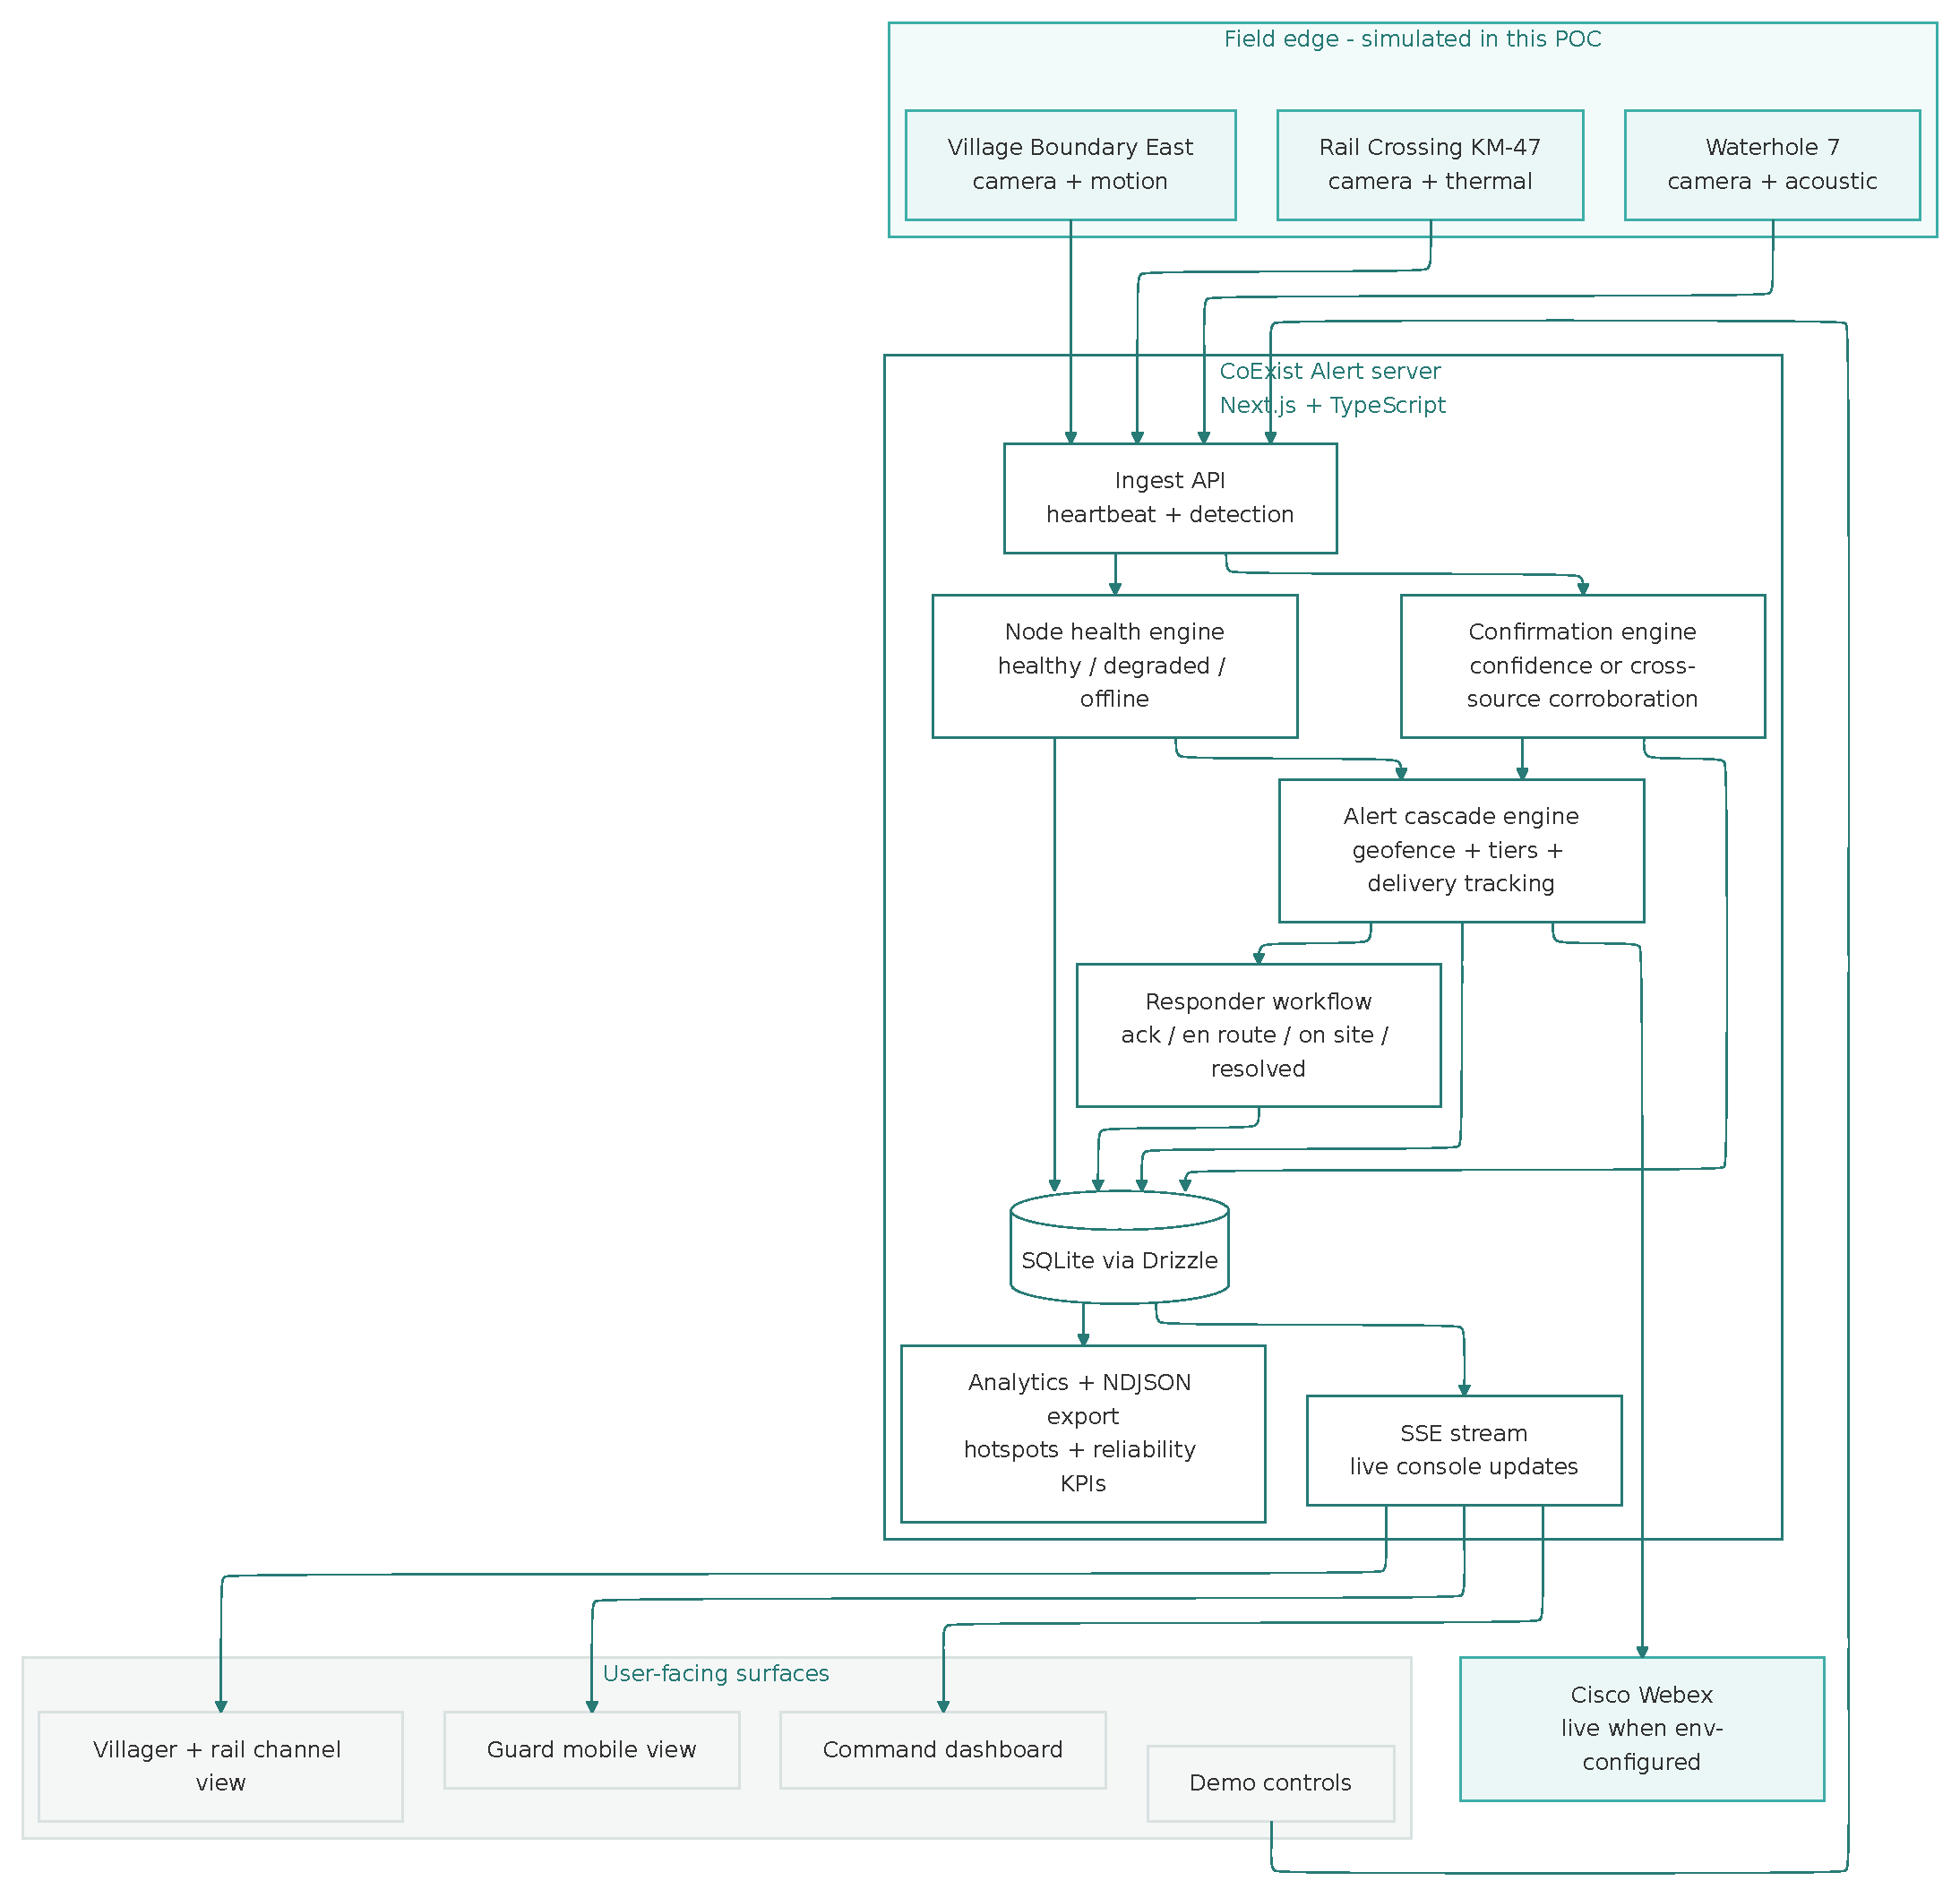
\includegraphics[width=1.12\textwidth,height=0.82\textheight,keepaspectratio]{diagrams/architecture-system.pdf}}
\end{center}

\clearpage
\begin{landscape}
\section{Detection To Warning Sequence}

\begin{center}
\makebox[\linewidth][c]{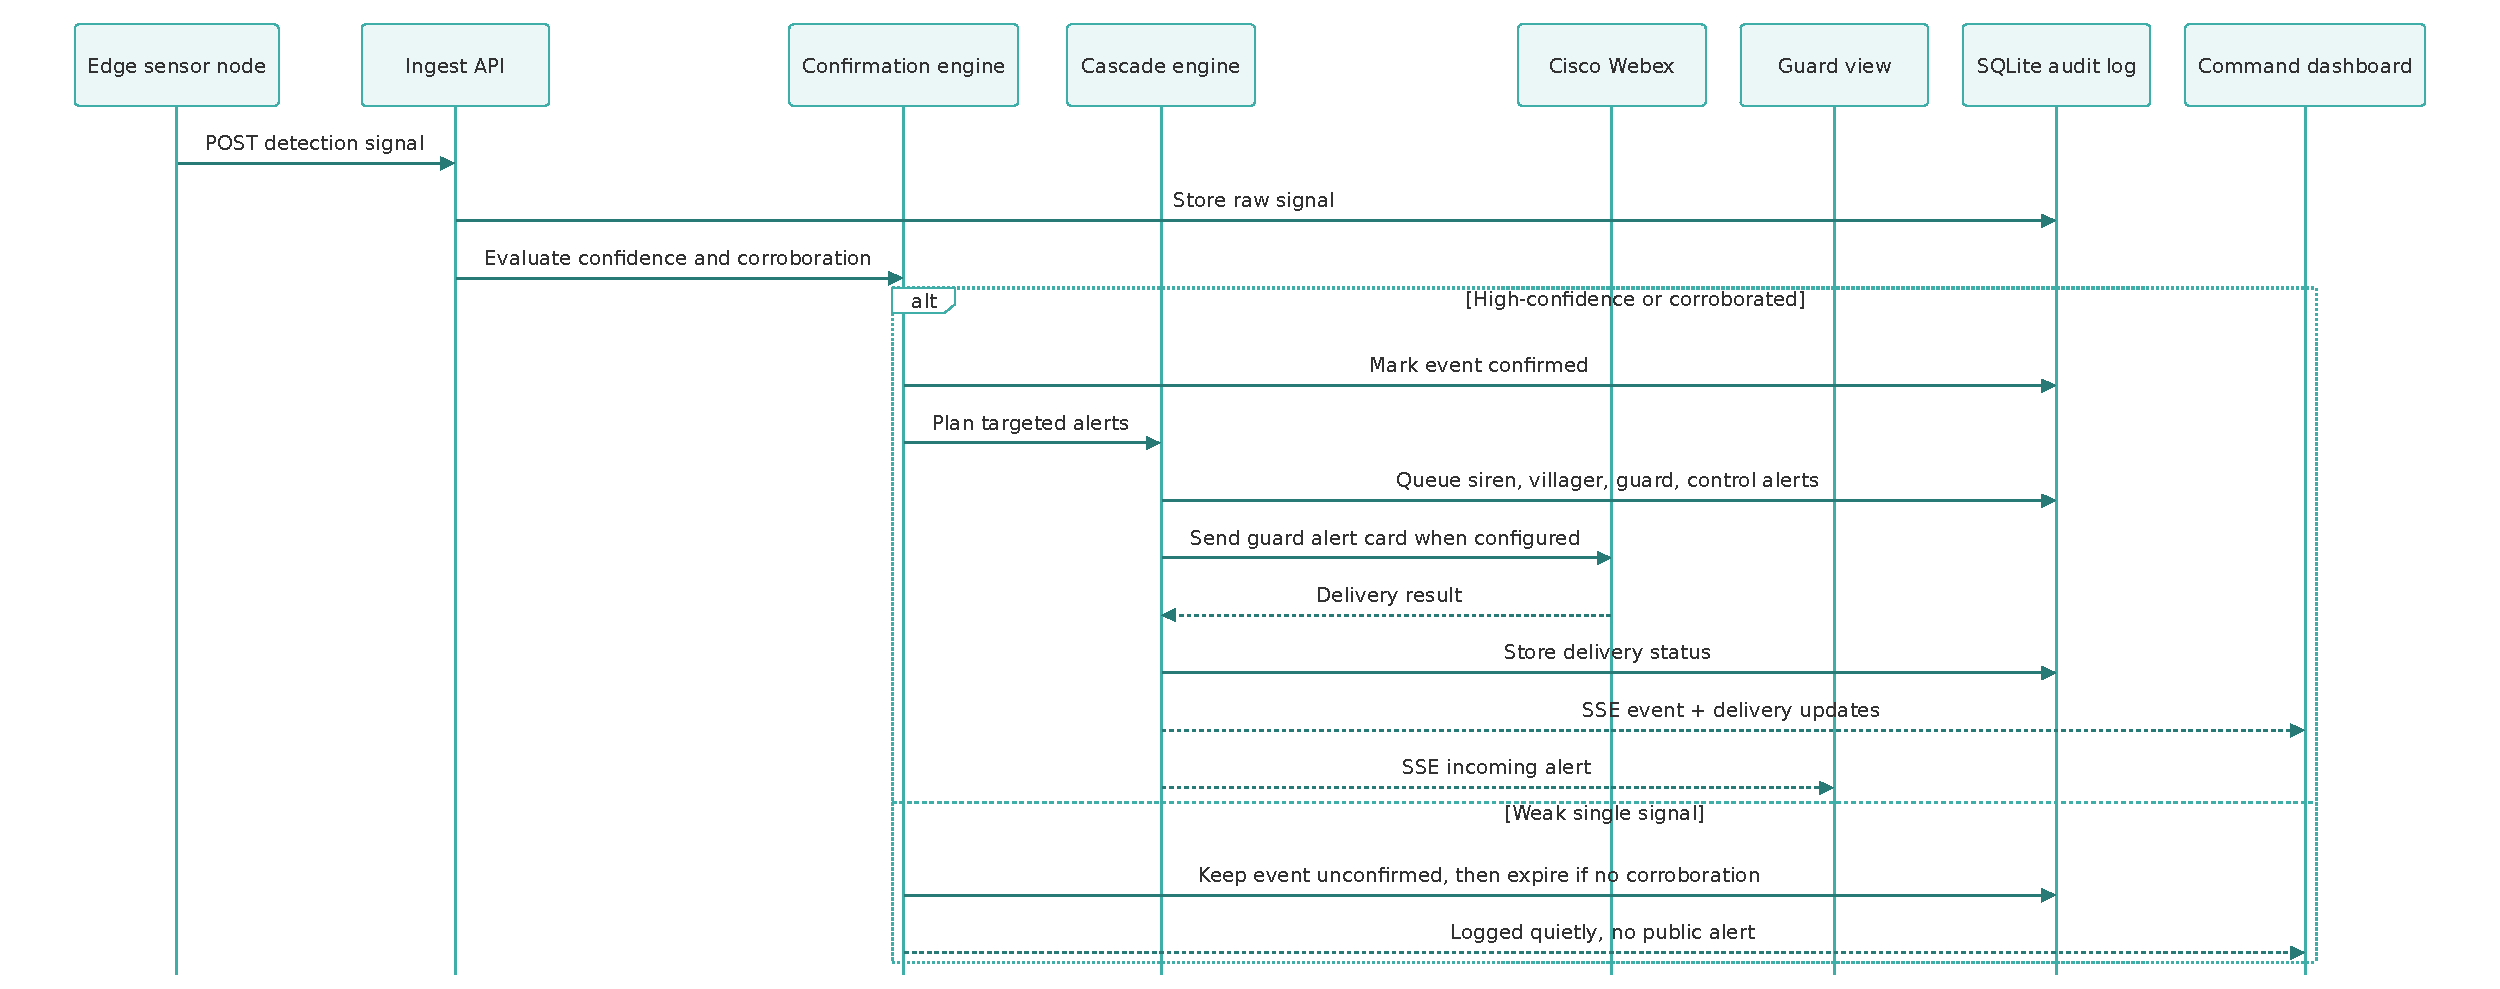
\includegraphics[width=1.12\linewidth,height=0.82\textheight,keepaspectratio]{diagrams/architecture-sequence.pdf}}
\end{center}
\end{landscape}

\clearpage
\section{Escalation And Ownership Workflow}

\begin{center}
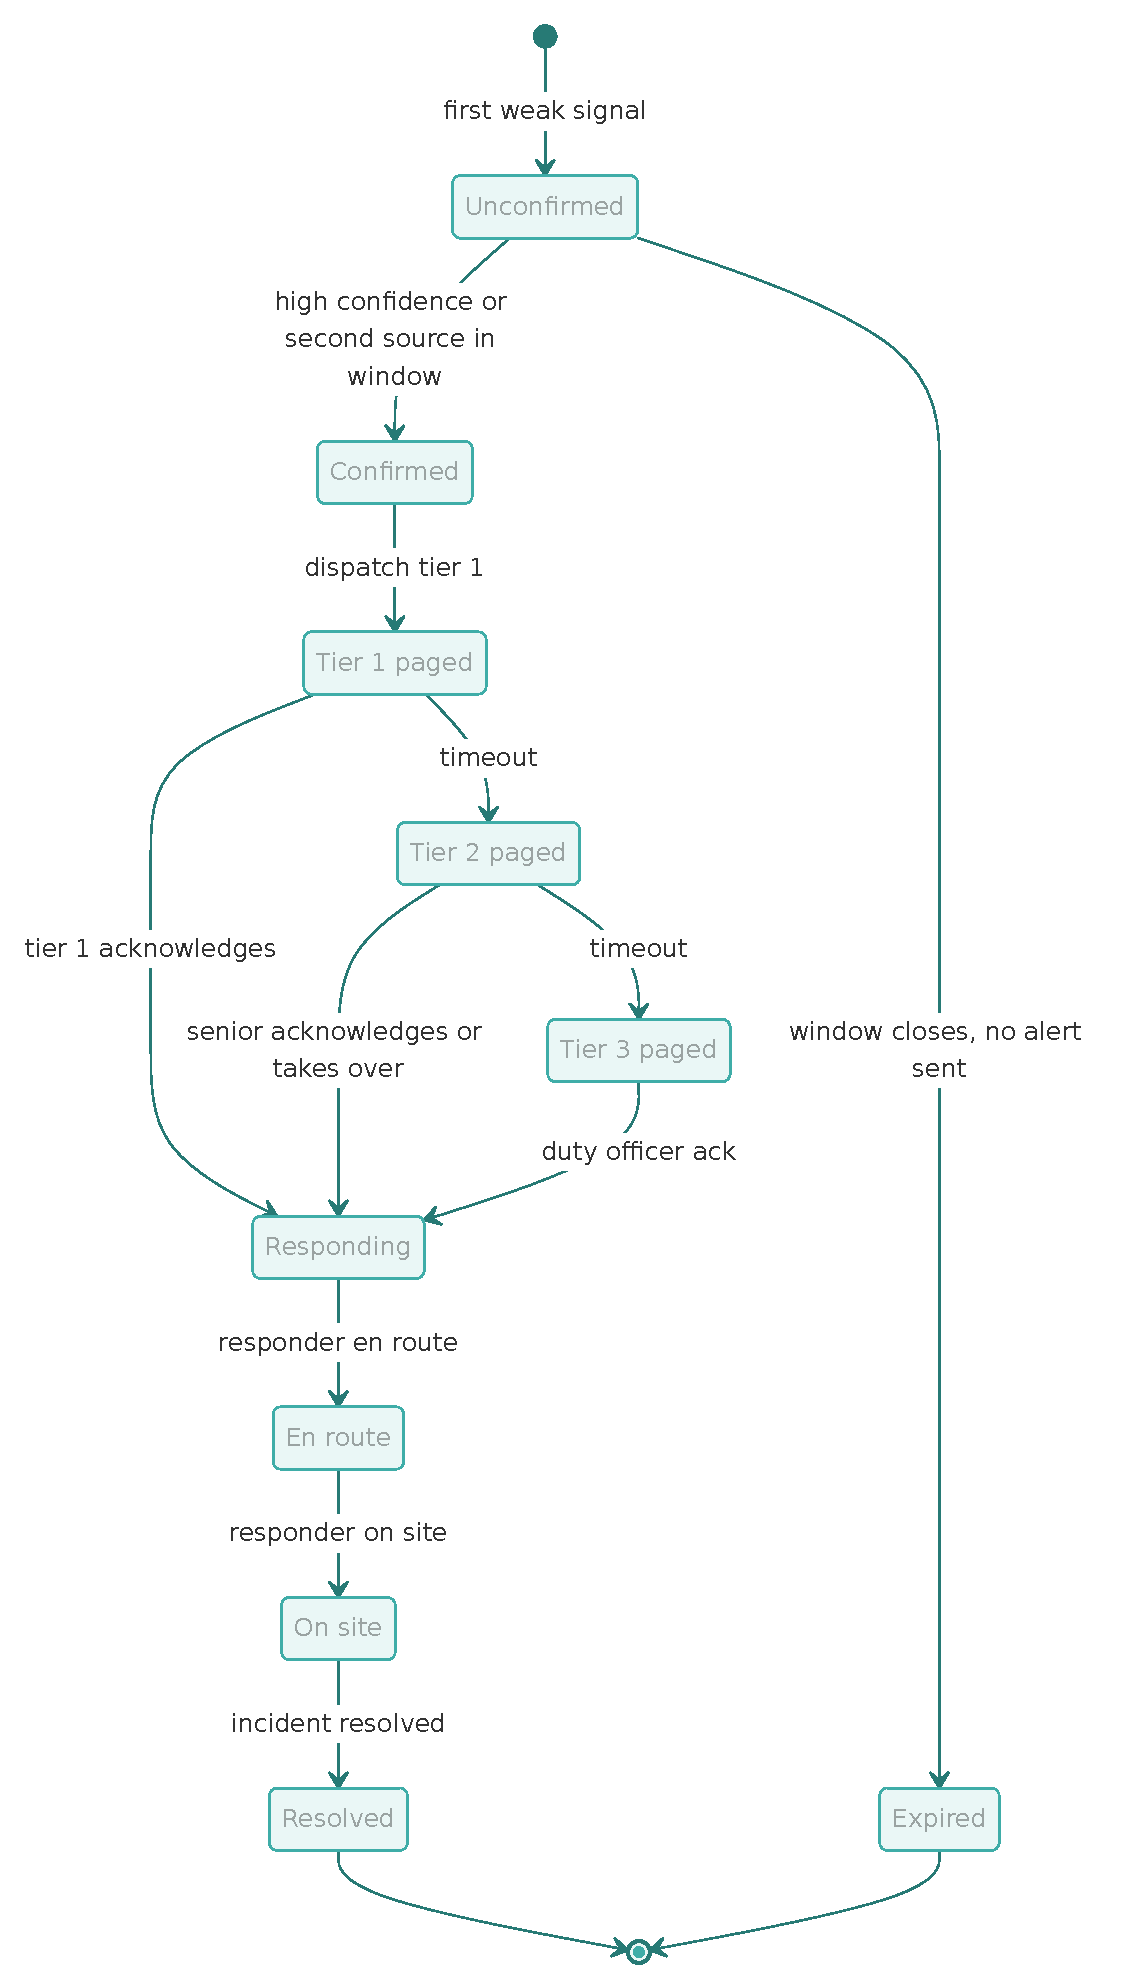
\includegraphics[width=0.96\textwidth,height=0.76\textheight,keepaspectratio]{diagrams/architecture-escalation.pdf}
\end{center}

\begin{decisionbox}{Ownership rule}
The first acknowledging responder owns the incident. A paged senior can take over, but other responders cannot progress or resolve someone else's active incident.
\end{decisionbox}

\clearpage
\section{Runtime And Deployment Flow}

\begin{center}
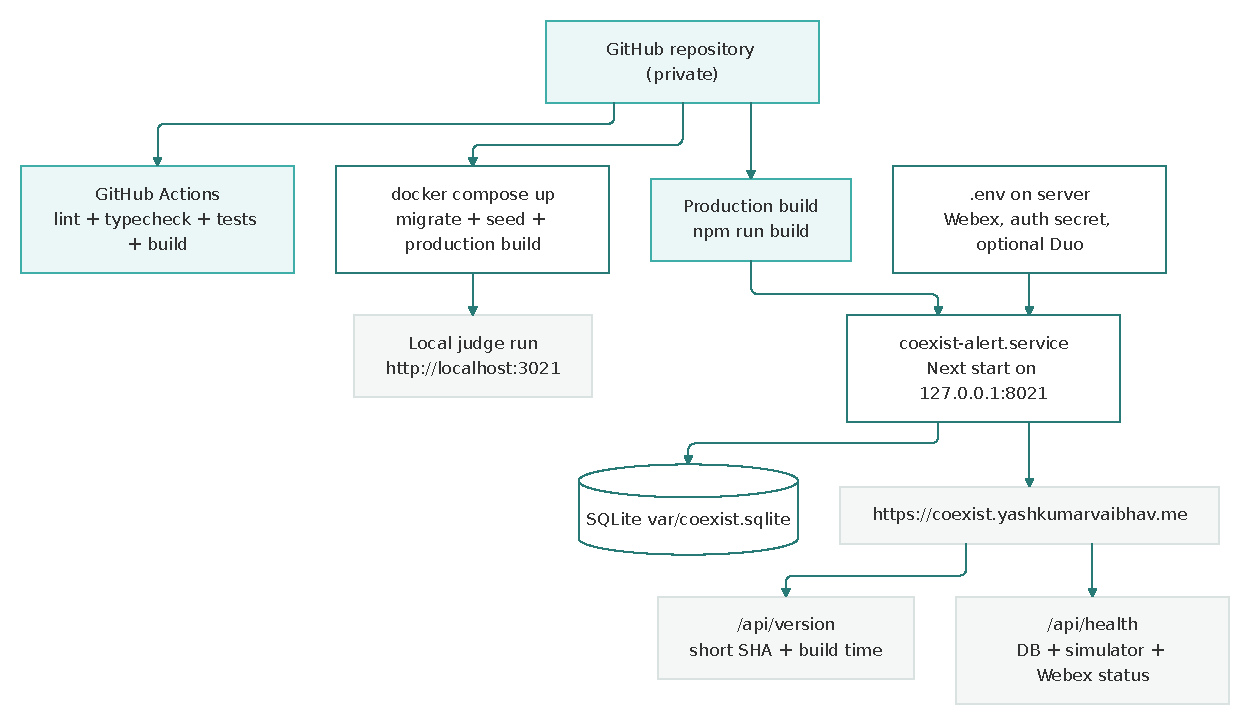
\includegraphics[width=0.96\textwidth,height=0.67\textheight,keepaspectratio]{diagrams/architecture-runtime.pdf}
\end{center}

\begin{decisionbox}{Deployment proof}
The public deployment is verified by matching the latest Git commit with \texttt{/api/version}, plus \texttt{/api/health} for database, simulator, and Webex readiness.
\end{decisionbox}

\clearpage
\section{Cisco Mapping Summary}

\begin{center}
\small
\begin{tabularx}{\textwidth}{@{}l l Y@{}}
\toprule
\textbf{Stage} & \textbf{Cisco product} & \textbf{Role in CoExist Alert} \\
\midrule
Sense & Meraki MV, MT, Cisco Spaces & Production edge detection and sensor payload shape. \\
Observe & ThousandEyes, Splunk & Health semantics, reliability analytics, event-log export. \\
Engage & Webex APIs & Live guard alert card and optional in-card acknowledgement. \\
Connect & Meraki MG, Catalyst & Remote backhaul narrative and link-quality model. \\
Secure & Duo, Secure Access, Umbrella & App auth/RBAC now; Duo step-up when configured; production access-control path. \\
\bottomrule
\end{tabularx}
\end{center}

\end{document}
